\documentclass{beamer}



\usepackage{verbatim}
\usepackage{fancyvrb}
\usepackage{color}

\newcommand\PYZat{@}
\newcommand\PYZlb{[}
\newcommand\PYZrb{]}
\newcommand\PYbh[1]{\textcolor[rgb]{0.00,0.50,0.00}{\textbf{#1}}}
\newcommand\PYbg[1]{\textcolor[rgb]{0.73,0.40,0.53}{\textbf{#1}}}
\newcommand\PYbf[1]{\textcolor[rgb]{0.82,0.25,0.23}{\textbf{#1}}}
\newcommand\PYbe[1]{\textcolor[rgb]{0.40,0.40,0.40}{#1}}
\newcommand\PYbd[1]{\textcolor[rgb]{0.73,0.13,0.13}{#1}}
\newcommand\PYbc[1]{\textcolor[rgb]{0.00,0.50,0.00}{\textbf{#1}}}
\newcommand\PYbb[1]{\textcolor[rgb]{0.00,0.50,0.00}{#1}}
\newcommand\PYba[1]{\textcolor[rgb]{0.00,0.00,0.50}{\textbf{#1}}}
\newcommand\PYaJ[1]{\textcolor[rgb]{0.69,0.00,0.25}{#1}}
\newcommand\PYaK[1]{\textcolor[rgb]{0.73,0.13,0.13}{#1}}
\newcommand\PYaH[1]{\textcolor[rgb]{0.50,0.00,0.50}{\textbf{#1}}}
\newcommand\PYaI[1]{\fcolorbox[rgb]{1.00,0.00,0.00}{1,1,1}{#1}}
\newcommand\PYaN[1]{\textcolor[rgb]{0.74,0.48,0.00}{#1}}
\newcommand\PYaO[1]{\textcolor[rgb]{0.00,0.00,1.00}{\textbf{#1}}}
\newcommand\PYaL[1]{\textcolor[rgb]{0.00,0.00,1.00}{#1}}
\newcommand\PYaM[1]{\textcolor[rgb]{0.73,0.73,0.73}{#1}}
\newcommand\PYaB[1]{\textcolor[rgb]{0.73,0.13,0.13}{#1}}
\newcommand\PYaC[1]{\textcolor[rgb]{0.67,0.13,1.00}{#1}}
\newcommand\PYaA[1]{\textcolor[rgb]{0.00,0.50,0.00}{#1}}
\newcommand\PYaF[1]{\textcolor[rgb]{0.63,0.00,0.00}{#1}}
\newcommand\PYaG[1]{\textcolor[rgb]{1.00,0.00,0.00}{#1}}
\newcommand\PYaD[1]{\textcolor[rgb]{0.00,0.50,0.00}{\textbf{#1}}}
\newcommand\PYaE[1]{\textcolor[rgb]{0.25,0.50,0.50}{\textit{#1}}}
\newcommand\PYaZ[1]{\textcolor[rgb]{0.00,0.50,0.00}{\textbf{#1}}}
\newcommand\PYaX[1]{\textcolor[rgb]{0.00,0.50,0.00}{#1}}
\newcommand\PYaY[1]{\textcolor[rgb]{0.73,0.13,0.13}{#1}}
\newcommand\PYaR[1]{\textcolor[rgb]{0.40,0.40,0.40}{#1}}
\newcommand\PYaS[1]{\textcolor[rgb]{0.10,0.09,0.49}{#1}}
\newcommand\PYaP[1]{\textcolor[rgb]{0.00,0.00,0.50}{\textbf{#1}}}
\newcommand\PYaQ[1]{\textcolor[rgb]{0.49,0.56,0.16}{#1}}
\newcommand\PYaV[1]{\textcolor[rgb]{0.00,0.00,1.00}{\textbf{#1}}}
\newcommand\PYaW[1]{\textcolor[rgb]{0.73,0.13,0.13}{#1}}
\newcommand\PYaT[1]{\textcolor[rgb]{0.40,0.40,0.40}{#1}}
\newcommand\PYaU[1]{\textcolor[rgb]{0.25,0.50,0.50}{\textit{#1}}}
\newcommand\PYaj[1]{\textcolor[rgb]{0.00,0.50,0.00}{#1}}
\newcommand\PYak[1]{\textcolor[rgb]{0.73,0.40,0.53}{#1}}
\newcommand\PYah[1]{\textcolor[rgb]{0.63,0.63,0.00}{#1}}
\newcommand\PYai[1]{\textcolor[rgb]{0.10,0.09,0.49}{#1}}
\newcommand\PYan[1]{\textcolor[rgb]{0.40,0.40,0.40}{#1}}
\newcommand\PYao[1]{\textcolor[rgb]{0.73,0.40,0.13}{\textbf{#1}}}
\newcommand\PYal[1]{\textcolor[rgb]{0.25,0.50,0.50}{\textit{#1}}}
\newcommand\PYam[1]{\textbf{#1}}
\newcommand\PYab[1]{\textit{#1}}
\newcommand\PYac[1]{\textcolor[rgb]{0.73,0.13,0.13}{#1}}
\newcommand\PYaa[1]{\textcolor[rgb]{0.50,0.50,0.50}{#1}}
\newcommand\PYaf[1]{\textcolor[rgb]{0.25,0.50,0.50}{\textit{#1}}}
\newcommand\PYag[1]{\textcolor[rgb]{0.40,0.40,0.40}{#1}}
\newcommand\PYad[1]{\textcolor[rgb]{0.00,0.25,0.82}{#1}}
\newcommand\PYae[1]{\textcolor[rgb]{0.40,0.40,0.40}{#1}}
\newcommand\PYaz[1]{\textcolor[rgb]{0.00,0.63,0.00}{#1}}
\newcommand\PYax[1]{\textcolor[rgb]{0.60,0.60,0.60}{\textbf{#1}}}
\newcommand\PYay[1]{\textcolor[rgb]{0.00,0.50,0.00}{\textbf{#1}}}
\newcommand\PYar[1]{\textcolor[rgb]{0.10,0.09,0.49}{#1}}
\newcommand\PYas[1]{\textcolor[rgb]{0.73,0.13,0.13}{\textit{#1}}}
\newcommand\PYap[1]{\textcolor[rgb]{0.00,0.50,0.00}{\textbf{#1}}}
\newcommand\PYaq[1]{\textcolor[rgb]{0.53,0.00,0.00}{#1}}
\newcommand\PYav[1]{\textcolor[rgb]{0.67,0.13,1.00}{\textbf{#1}}}
\newcommand\PYaw[1]{\textcolor[rgb]{0.40,0.40,0.40}{#1}}
\newcommand\PYat[1]{\textcolor[rgb]{0.10,0.09,0.49}{#1}}
\newcommand\PYau[1]{\textcolor[rgb]{0.10,0.09,0.49}{#1}}








% own commands
\newcommand{\pv}{\pause \vspace{1ex}}

\newcommand{\tbf}{\textbf}
\newcommand{\tsc}{\textsc}
\newcommand{\Ra}{\Rightarrow}
\newcommand{\La}{\Leftarrow}
\newcommand{\agn}{\leftarrow}
\newcommand{\nat}{\mathbb{N}}
\newcommand{\natn}{\mathbb{N}_0}
\newcommand{\Ree}{\mathbb{R}}
\newcommand{\Rn}{\mathbb{R}^n}
\newcommand{\Rm}{\mathbb{R}^m}
\newcommand{\Rmn}{\mathbb{R}^{m \times n}}
\newcommand{\Gr}{$G = (V,E)$ }
\newcommand{\gGr}{$D = (V,E)$ }
\newcommand{\Gwfkt}{$c: E \rightarrow \mathbb{R}$ }
\newcommand{\Gwfktp}{$c: E \rightarrow \mathbb{R}_0^+$ }
\newcommand{\Gwfktg}{$c: E \rightarrow \mathbb{N}_0$ }
\newcommand{\Gwfktn}{$c: E \rightarrow \mathbb{N}$ }
\newcommand{\Cut}{$(S,V \setminus S)$ }
\newcommand{\Lra}{\Leftrightarrow}
\newcommand{\Nw}{$(D;s,t;c)$ }
\newcommand{\Flu}{$f: E \rightarrow \mathbb{R}_0^+$ }
\newcommand{\Flue}{$f: E' \rightarrow \mathbb{R}$ }
\newcommand{\NP}{\mathcal{NP}}
\newcommand{\NPC}{\mathcal{NPC}}
\newcommand{\RP}{\mathcal{RP}}
\newcommand{\PP}{\mathcal{PP}}
\newcommand{\BPP}{\mathcal{BPP}}
\renewcommand{\Pr}{\text{Pr}}
\newcommand{\NC}{\mathcal{NC}}
\newcommand{\SC}{\mathcal{SC}}
\newcommand{\FPT}{\mathcal{FPT}}


\newcommand{\calA}{\mathcal{A}}
\newcommand{\calB}{\mathcal{B}}
\newcommand{\calC}{\mathcal{C}}
\newcommand{\calF}{\mathcal{F}}
\newcommand{\calH}{\mathcal{H}}
\newcommand{\calK}{\mathcal{K}}
\newcommand{\calL}{\mathcal{L}}
\newcommand{\calP}{\mathcal{P}}
\newcommand{\calR}{\mathcal{R}}
\newcommand{\calU}{\mathcal{U}}


\newcommand{\isep}{\addtolength{\itemsep}{0.25\baselineskip}}
\newcommand{\isepp}{\addtolength{\itemsep}{0.125\baselineskip}}

%\usepackage[ngerman]{babel}
\usepackage[utf8]{inputenc}
\usepackage[T1]{fontenc}
\usepackage{amsmath}
\usepackage{amssymb}
\usepackage{amsthm}
\usepackage{tikz}

\usepackage[usenames,dvipsnames]{pstricks}
\usepackage{epsfig}
\usepackage{pst-grad} % For gradients
\usepackage{pst-plot} % For axes


\usepackage{float}
\usepackage{algorithm}
\usepackage[noend]{algorithmic}
\floatname{algorithm}{Algorithmus}
\renewcommand{\listalgorithmname}{Liste der Algorithmen}
\newcommand{\Eingabe}[1]{\STATE \tbf{Eingabe}: #1 \\}
\newcommand{\Ausgabe}[1]{\STATE \tbf{Ausgabe}: #1 \\}
\newcommand{\Seffekte}[1]{\STATE \tbf{Seiteneffekte}: #1 \\}
\newcommand{\Vorb}[1]{\STATE \tbf{Vorbedingungen}: #1 \\}
\renewcommand{\algorithmicif}{\textbf{Falls}}
\renewcommand{\algorithmicthen}{}
\renewcommand{\algorithmicelse}{\textbf{Sonst}}
\renewcommand{\algorithmicwhile}{\textbf{Solange}}
\renewcommand{\algorithmicdo}{}
\renewcommand{\algorithmicfor}{\textbf{Für}}
\renewcommand{\algorithmicforall}{\textbf{Für alle}}
\definecolor{mygray}{gray}{.20}
\renewcommand{\algorithmiccomment}[1]{\textcolor{mygray}{ // #1}}

\usepackage{stmaryrd}



\usetheme{Singapore}
\usecolortheme{seahorse}
\usecolortheme{rose}
\setbeamercovered{invisible}
\beamertemplatenavigationsymbolsempty
\setbeamertemplate{footline}[frame number]
\setbeamertemplate{theorems}[numbered]
%\setbeamertemplate{navigation symbols}{}

\setlength{\parindent}{0pt}
\setcounter{topnumber}{1}

%\renewcommand{\qedsymbol}{\ }
%\theoremstyle{default}
\newtheorem{satz}[theorem]{Satz}
%\newtheorem{behauptung}{Behauptung}

% \usepackage{setspace}
% \onehalfspacing
\renewcommand{\baselinestretch}{1.25}

\definecolor{darkblue}{rgb}{0,0,.5}


% \newenvironment{Ventry}[1]%
% {\begin{list}{}{\renewcommand{\makelabel}[1]{\textsf{##1:}\hfil}%
% \settowidth{\labelwidth}{\textsf{#1:}}%
% \setlength{\leftmargin}{\labelwidth + \labelsep}}}%
% {\end{list}}

\mode<presentation>

% shadow of not yet presented items
\setbeamercovered{invisible}
\beamertemplatenavigationsymbolsempty

% View structure of presentation before new section
% \AtBeginSection[]
% {
%   \begin{frame}<beamer>{AspectJ}
%     \tableofcontents[currentsection,currentsubsection]
%   \end{frame}
% }

% \AtBeginSubsection[]
% {
%   \begin{frame}<beamer>{AspectJ}
%     \tableofcontents[currentsection,currentsubsection]
%   \end{frame}
% }


\begin{document}
\title{McLab and AspectMatlab}
\subtitle{\small{A Domain Specific Extensible Compiler Framework and
    Example Extension}}

\author{Jesse Doherty\\Anton Dubrau} 
\date{Some date?} 


\small
\setbeamerfont{block title}{size=\small}
\setbeamerfont{frametitle}{size=\normalsize}

\frame{\titlepage} 

%\frame{\frametitle{AspectJ}\tableofcontents[pausesections,pausesubsections]} 
\frame{\frametitle{McLab}\tableofcontents} 

% \section{Introduction}
% \subsection{McLab!!!}
% \begin{frame}
% McLab is awesome!
% \end{frame}
% \begin{frame}
%   \begin{block}{foo block title?}
%     foo
%   \end{block}
%   \begin{block}{bar block title?}
%     bar
%   \end{block}
% \end{frame}
% \begin{frame}
%   \begin{itemize}
%   \item this is a bullet list
%   \end{itemize}
% \end{frame}

\section{McLab}
\subsection{Project Goal}
\begin{frame}{Project Goal}
  %\begin{center}
    \begin{onlyenv}<1>
      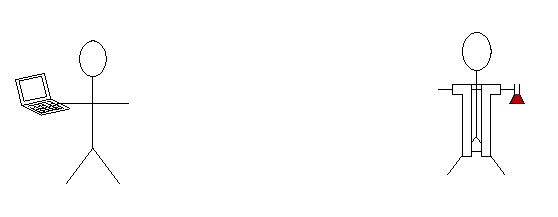
\includegraphics{images/perspectives1.pdf}
    \end{onlyenv}
    \begin{onlyenv}<2>
      
\includegraphics{images/perspectives2_comp.pdf}
    \end{onlyenv}
    \begin{onlyenv}<3>
      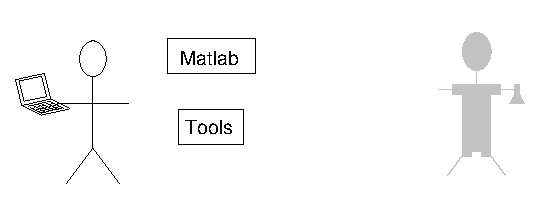
\includegraphics{images/perspectives3_comp.pdf}
    \end{onlyenv}
    \begin{onlyenv}<4>
      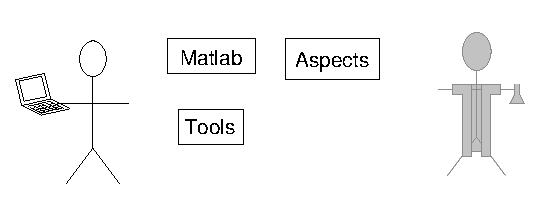
\includegraphics{images/perspectives4_comp.pdf}
    \end{onlyenv}
    \begin{onlyenv}<5>
      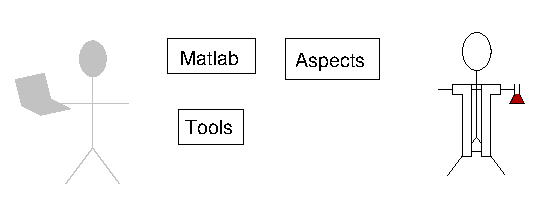
\includegraphics{images/perspectives5_sci.pdf}
    \end{onlyenv}
    \begin{onlyenv}<6>
      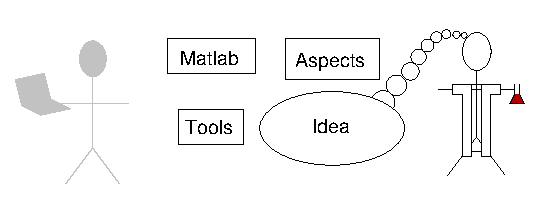
\includegraphics{images/perspectives6_sci.pdf}
    \end{onlyenv}
    \begin{onlyenv}<7>
      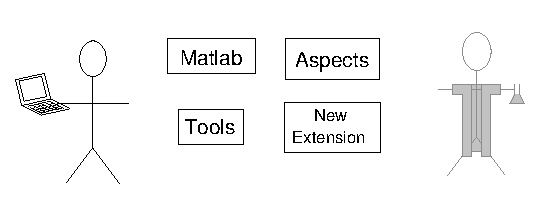
\includegraphics{images/perspectives7_comp.pdf}
    \end{onlyenv}
    \begin{onlyenv}<8>
      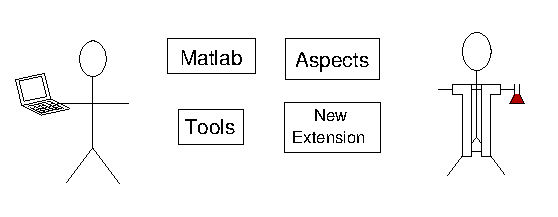
\includegraphics{images/perspectives_base.pdf}
    \end{onlyenv}
  %\end{center}
\end{frame}

\subsection{Overall Structure}
\begin{frame}{The Mclab system and AspectMatlab}
  \begin{center}
    \only<1>{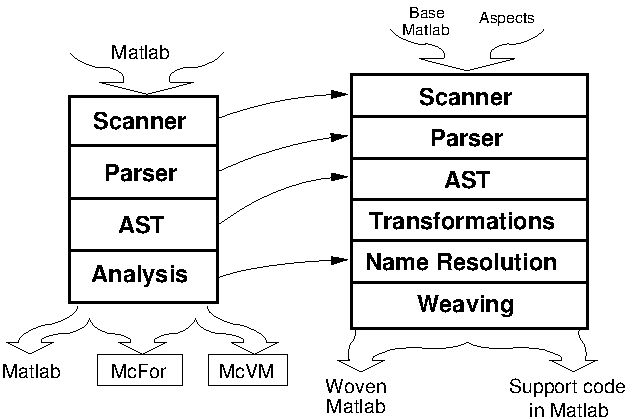
\includegraphics[scale=0.9]{images/mclab_aspect_full.pdf}}
    \only<2>{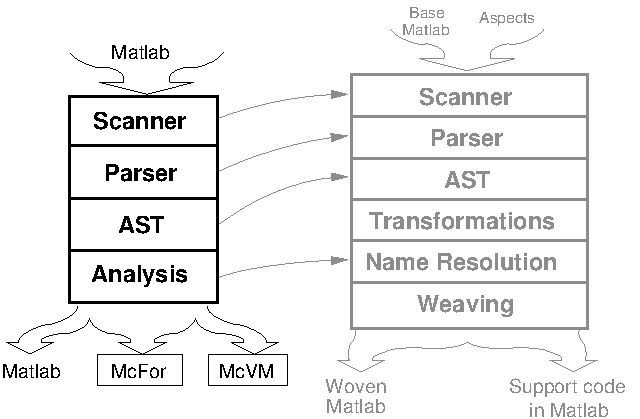
\includegraphics[scale=0.9]{images/mclab_aspect_mclab.pdf}}
  \end{center}

\end{frame}

\section{Extensible design}
\begin{frame}[t]{Extensible design}
  \begin{columns}[T]
    \begin{column}{5cm}
      \only<1>{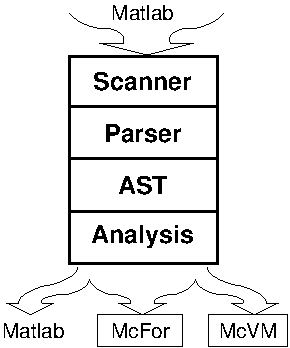
\includegraphics{images/mclab_plain.pdf}}
      \only<2>{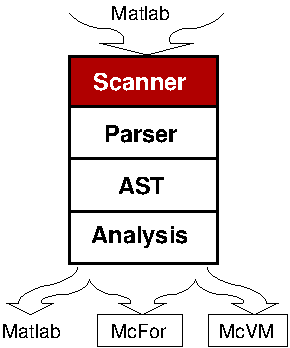
\includegraphics{images/mclab_scanner.pdf}}
      \only<3>{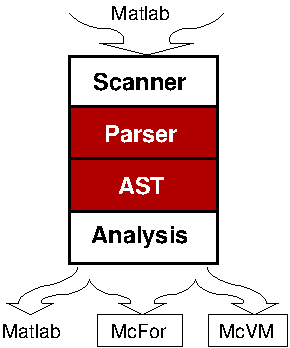
\includegraphics{images/mclab_jastadd.pdf}}
      \only<4>{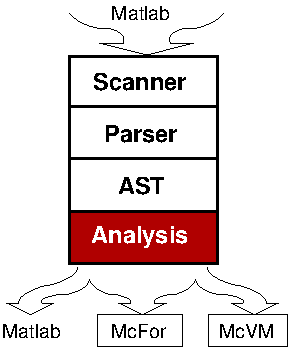
\includegraphics{images/mclab_analysis.pdf}}
    \end{column}
    \begin{column}{5cm}
      \begin{onlyenv}<1>
        \begin{block}{Domain-specific extensions}
          \begin{itemize}
          \item New data structure capabilities
          \item New control flow
          \item Different language constructs
          \end{itemize}
        \end{block}
      \end{onlyenv}
      \begin{onlyenv}<2>
        \begin{block}{Metalexer {\tiny[Casey MSc McGill `09]}
          \vspace{1ex}}
          \begin{center}
            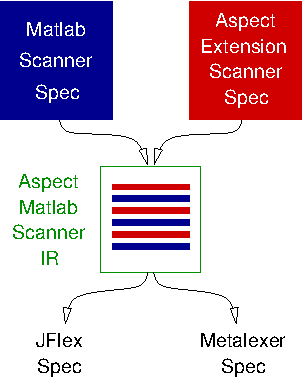
\includegraphics[scale=0.7]{images/metalexer.pdf}
          \end{center}

        \end{block}
      \end{onlyenv}
      \begin{onlyenv}<3>
        \begin{block}{JastAdd {\tiny[Ekman, Hedin SCP `07]}}
          \begin{itemize}
          \item JastAdd parser generator
          \item JastAdd 
            \begin{itemize}
            \item Extensible AST specification
            \item Attribute grammar
            \item Specialized aspect system
            \item Used in abc
            \end{itemize}
          \end{itemize}
        \end{block}
      \end{onlyenv}
      \begin{onlyenv}<4>
        \begin{block}{Analysis framework \\{\tiny[Doherty MSc McGill `10]}}
          \begin{itemize}
          \item Extendable to new language features
          \item Use existing analyses in extensions
          \end{itemize}
        \end{block}
      \end{onlyenv}
    \end{column}
  \end{columns}
\end{frame}
\begin{frame}[t]{Analysis framework}
  \begin{columns}[T]
    \begin{column}{4cm}
      \begin{block}{Base framework}
        \begin{center}
          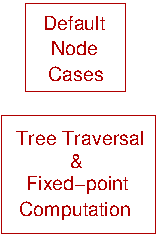
\includegraphics{images/analysis_left.pdf}
        \end{center}
      \end{block}
    \end{column}
    \begin{column}{6cm}
      \begin{onlyenv}<2>
        \begin{block}{A new analysis}
          \begin{center}
            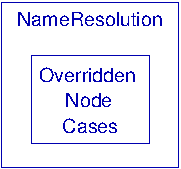
\includegraphics{images/analysis_right.pdf}
          \end{center}
        \end{block}
      \end{onlyenv}
      \begin{onlyenv}<3->
        \begin{block}{Extensions: 
            \only{no new analyses or important nodes}<3>
            \only{no important nodes}<4>
            \only{new structural nodes}<5>
          }
          \begin{center}
            \begin{onlyenv}<3>
              Handled by class hierarchy and default cases
            \end{onlyenv}
            \begin{onlyenv}<4>
              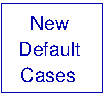
\includegraphics{images/analysis_extension2.pdf}
            \end{onlyenv}
            \begin{onlyenv}<5>
              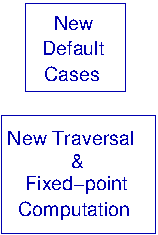
\includegraphics{images/analysis_extension3.pdf}
            \end{onlyenv}
          \end{center}
        \end{block}
      \end{onlyenv}
    \end{column}
  \end{columns}
  
\end{frame}

\section{Aspect Matlab}

\subsection*{AspectMatlab introduction}

\begin{frame}{Matlab Extensions}
  \begin{center}
    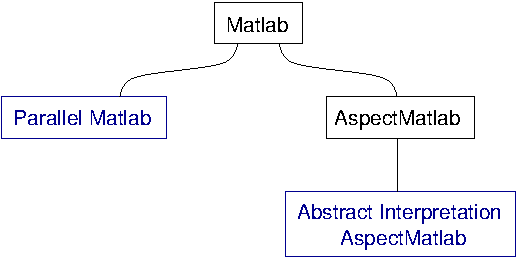
\includegraphics{images/extensions.pdf}
  \end{center}
\end{frame}
\begin{frame}{AspectMatlab: an Matlab extension}
  \begin{center}
    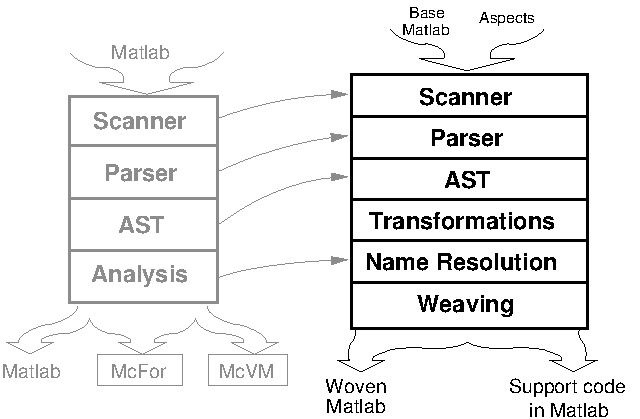
\includegraphics[scale=0.9]{images/mclab_aspect_aspect.pdf}
  \end{center}

\end{frame}


\section{Anton applications}



\section{Domain specific challenges}
\begin{frame}
d
\end{frame}
\section{Anton examples }
\begin{frame}{Why Aspect Matlab?}
  \begin{onlyenv}<1-2>
    An aspect extension to Matlab seems odd:
    \begin{itemize}
    \item Matlab programs are small % even with libraries
    \item Scientific computing doesn't rely on classes
    \end{itemize}
    \uncover<2>{
      \vspace{4ex}
      \begin{itemize}
      \item What is the domain of Aspect Matlab?
      \end{itemize}  
    }
  \end{onlyenv}
  \begin{onlyenv}<3-4>
    % i was basically given the existing language and compiler and told
    % hey, you've taking some numerical classes, figure out how this is useful.     
    % let's look at matlab's domain...
    \begin{itemize}
    \item Matlab's domain:
      \begin{itemize}
      \item Numerical/scientific computing
      \end{itemize}
    % ...and what are the core issues to programmers
    \uncover<4>{
    \item Issues
      \begin{itemize}
      \item Performance/high productivity
        \begin{itemize}
        \item Matlab's libraries are fast, the language is easy
        \item Dynamic features may cause slow execution
        \end{itemize}
      \item Domain specific extra functionality
        \begin{itemize}
        \item Hundreds of toolboxes
        \end{itemize}
      \end{itemize}
    }
    \end{itemize}
  \end{onlyenv}
  \begin{onlyenv}<5>
    Aspect matlab domain
    \begin{itemize}
    \item Leverage these domains (performance, extensions)
      \begin{itemize}
      \item Reusable aspects that help increase performance
        by domain specific profiling
      \end{itemize}
    \item Domain specific extensions
      \begin{itemize}
      \item We can use aspects to extend functionality
      \end{itemize}
    \end{itemize}
  \end{onlyenv}
\end{frame}


\subsection*{Profiling}
% intro
%  profiling
% matlab has fast libraries, but the language has a lot of bottlenecks
% having a lot of detailed knowledge about one's program can help speed up performance
% the aspect matlab language allows for very detailed pointcuts
% before, around, after calling functions, setting and getting arrays
% and provides a lot of context information for every shadow (?)
% -- more on that in the actual talk on x

% we can write reusable aspects that profile very specific properties
% of a program
% examples:
\begin{frame}{Profiling Aspects}



  \begin{itemize}
\item Pointcuts get/set/call % allow very detailed view of whats going on
\item A lot of context info  %all the context information provides even more info at the same time
\item Performance is important in this domain
\begin{itemize}
\item More knowledge improves performance
\end{itemize}
%\item --> it's a domain where you want to know exactly what's going on in your program
\end{itemize}
\end{frame}
% flops 1
\begin{frame}[fragile]{Profiling I - Flops}
  \begin{onlyenv}<1-4>
    % let's say as a scientist/engineer i want to know where most
    % compuations happens
    % since my program is all matrizes, most of the program is spent doing
    % matrix operations
    % the basic unit of computational complexity is the floating point
    % operation -- tend to be the most numerous and expensive part of a
    % program -- numerical algorithms are counted and analyzed in flops
    \vspace{4ex}
    \begin{itemize}
    \item where does computation happen?
    \pause \item most of the program - matrix computations
    \pause \item basic unit of that - flop
      \begin{itemize}
      \item most expensive and numerous
      \item we count/analyze programs in flops
      \end{itemize}
    \pause \item goal: an aspect that tells us the total flops
    \end{itemize}
  \end{onlyenv}
    \begin{columns}
      \begin{column}[T]{5cm}
        \begin{onlyenv}<5>
          \begin{Verbatim}[commandchars=@\[\]]
aspect flops
  ...
  patterns
    pplus : call(plus)
    pmul  : call(mtimes)
    ...
  end

  actions
    ...
  end
end
        \end{Verbatim}
      \end{onlyenv}
        \begin{onlyenv}<6>
          \begin{Verbatim}[commandchars=@\[\]]
aspect flops
  ...
  patterns
    @PYaG[pplus : call(plus)]
    @PYaG[pmul  : call(mtimes)]
    ...
  end

  actions
    ...
  end
end
        \end{Verbatim}
      \end{onlyenv}
        \begin{onlyenv}<7>
          \begin{Verbatim}[commandchars=@\[\]]
actions
  around pplus : 
    @PYaG[this.flops = this.flops + ..]
      @PYaG[numel(args{1})]
  end
        
  before pmtimes : (args)
    [m,n] = size(args{1})
    [n,k] = size(args{2})
    @PYaG[this.flops = this.flops+2*m*n*k]
  end
end
        \end{Verbatim}
      \end{onlyenv}
        \begin{onlyenv}<8>
          \begin{Verbatim}[commandchars=@\[\]]
actions
  around pplus : 
    this.flops = this.flops + ..
      numel(args{1})
  end
        
  before pmtimes : (args)
    @ob[]m,n@cb = size(args{1})
    @ob[]n,k@cb = size(args{2})
    this.flops = this.flops+2*m*n*k
  end
end
        \end{Verbatim}
      \end{onlyenv}
      \end{column}
      \begin{column}[T]{5cm}
        \begin{itemize}
          \pause \item We catch all operations
          \pause \pause \item In befores we add up estimated flops
          \pause \item We display result at the end
            % this can be done in core matlab - but involves some
            % hackery. also aspects allows this to be in one file,
            % much shorter and easier
        \end{itemize}
      \end{column}
    \end{columns}


  % so we want to write an aspect that tells us how many flops
  % every operation takes

  % start left/right
  % we simply overrade all operations (show aspect code overriding operations)
  % and in the operations we can add up an estimate for computational of
  % the flops (show advice adding stuff)
\end{frame}

% flops 2
\begin{frame}[fragile]{Profiling II - Flops Extended}
  \begin{onlyenv}<1>
    \begin{itemize}
    \item Suppose now we want to know where these flops occur
    \item For every function, we want to know
      \begin{itemize}
      \item All flops that occur inside it
      \item How often it gets called
      \end{itemize}
    \end{itemize}
  \end{onlyenv}
  \begin{onlyenv}<2>
\begin{Verbatim}
   'call site'                'number of calls' 'total flops'
   'bar_3_mtimes                 [        40] [       4000]
   'bar_5_plus                   [        20] [        200]
   'foo_3_mtimes'                [         5] [        800]
   'foo_4_bar'                   [         5] [       5000]
   'Script_1_foo'                [         1] [       5000]
\end{Verbatim}
  \end{onlyenv}
  \begin{onlyenv}<3->
    \begin{itemize}
    \pause
    \pause \item Now we don't only intercept Operators, but also function calls
    \pause \item We keep track of the flops in a stack
    \pause \item Before any function call we push 0
    \pause \item Around any operation (*,+,..) we
      \begin{itemize}
      \item Add estimated flops to top of stack
      \end{itemize}
    \pause \item After call we pop the value and
      \begin{itemize}
      \item Record the number of flops
      \item Add that number to the new top
      \end{itemize}    
      % in plain matlab, this is not possible without extensively
      % modifying the original code
    \end{itemize}
  \end{onlyenv}
\end{frame}

% flops 3
%\begin{frame}{Profiling III - interval arithmetic}
%  \begin{itemize}
%  \item lets go deeper into acally changing the original program
%  \item supposse we want upper ad lower bounds on numerical errors
%  (precision)
%  \item we can override all variables to be a structure including the
%  original value and the new annotated information
%  \item diagram (var) --> structure: value, some tag, annotated info
%  ---- should this actually be a class???
%  \item 
%  \end{itemize}
%\end{frame}


\subsection*{Extending Functionality}
\begin{frame}{Extending Functionality}
  Extending Functionality
  \begin{itemize}
  \item We have an extensible toolkit (McLab)
  \item We can use aspects for rapid prototyping of domain specific extensions
  \item We can use aspects to add new functionality % special libraries
  \end{itemize}
\end{frame}

\begin{frame}[fragile,t]{Extending Functionality I}
  \begin{columns}[T]
    \begin{column}{5cm}
      \begin{onlyenv}<2>
        \begin{Verbatim}[commandchars=@\[\]]
function y=plotThis(f,x)
  y = empty
  for t = x
    y = @ob[]y; f(t)@cb[]
  end
  plot(x,y)
end
        \end{Verbatim}
      \end{onlyenv}
      \begin{onlyenv}<3>
        \begin{Verbatim}[commandchars=@\[\]]
function y=plotThis(f,x)
  y = @PYaG[x]
  for t = x
    @PYaG[y(i) = f(t)]
  end
  plot(x,y)
end
        \end{Verbatim}
          \end{onlyenv}
          \begin{onlyenv}<4>
        \begin{Verbatim}[commandchars=@\[\]]
function y=plotThis(f,x)
  y = x
  for t = x
    y(@PYaG[i]) = f(t)
  end
  plot(x,y)
end
        \end{Verbatim}
          \end{onlyenv}
          \begin{onlyenv}<5>
        \begin{Verbatim}[commandchars=@\[\]]
function y=plotThis(f,x)
  y = x
  for @PYaG[@ob[]t,i@cb] = x
    y(@PYaG[i]) = f(t)
  end
  plot(x,y)
end
        \end{Verbatim}
          \end{onlyenv}
          \begin{onlyenv}<6-10>
        \begin{Verbatim}[commandchars=@\[\]]
function y=plotThis(f,x)
  y = x
  for t = x
    y(@PYaG[iteration()]) = f(t)
  end
  plot(x,y)
end
        \end{Verbatim}
          \end{onlyenv}
          \begin{onlyenv}<11>
        \begin{Verbatim}[commandchars=@\[\]]
function y=plotThis(f,x)
  y = x
  for t = x
    y(@PYaG[iteration]) = f(t)
  end
  plot(x,y)
end
        \end{Verbatim}
          \end{onlyenv}
      \end{column}

      \begin{column}{5cm}
        \begin{onlyenv}<1-5>
          \begin{itemize}
          \item<1-5> Consider our original example
          \item<2-5> We don't want to grow the array
          \item<4-5> Now we need to now i
          \item<5> We propose a language extension 
          \end{itemize}
        \end{onlyenv}
        \begin{onlyenv}<6-11>
          \begin{itemize}
          \item<6-11> Via an aspect we simply add an iteration() function
          \item<7-11> Capture all loops
          \item<8-11> Store context info in loop advice 
           \item<10-11> Return that in an around for a call to 'iteration'
          \item<11> 'iteration' returns the count
          \end{itemize}
        \end{onlyenv}
    \end{column}
  \end{columns}
\end{frame}




\begin{frame}[fragile,t]{Extending Functionality II - Units}
  \begin{itemize}
  \item Consider new addition of units
  \end{itemize}
  \begin{onlyenv}<2->
    \begin{Verbatim}
      bmi = 180*lb/(5*feet + 8*inches)^2
      v = 374*km / ((16*h+07*min)-(13*h+16*min))
      t = AU/c
    \end{Verbatim}
  \end{onlyenv}
  \begin{itemize}
    \pause
    \pause \item We have to
    \begin{itemize}
      \pause \item Annotate (override) all data
      \pause \item Override all operations
      \pause \item Override loops to restore the semantics
      \pause \item Capture all calls to units
    \end{itemize}
  \end{itemize}
\end{frame}


\begin{frame}[fragile,t]{Extending Functionality II - Units}
\begin{columns}[T]
  \begin{column}{10cm}
    \begin{itemize}
      \only{ \item We don't define a pattern for every unit.}<1->
      \only{ \item We simply keep a list of units...}<2->
      \only{ \item ..and constants.}<3->
      \only{ \item We match all calls with 0 arguments.}<4->
      \only{ \item We override them only if they are in the lists.}<5->
      \only{ \item We can still use unit names as variables.}<6->
    \end{itemize}
    \begin{onlyenv}<2>
      \begin{Verbatim}[commandchars=@\[\]]
  units = struct(...
    'm',  @ob1, 0, 0, 0, 0, 0, 0@cb[],...
    'Kg', @ob0, 1, 0, 0, 0, 0, 0@cb[],...
    ...
    'J',  @ob2, 1,-2, 0, 0, 0, 0@cb[],...
    'N',  @ob1, 1,-2, 0, 0, 0, 0@cb[]),
    ...
        \end{Verbatim}
      \end{onlyenv}
    \begin{onlyenv}<3>
      \begin{Verbatim}[commandchars=@\[\]]
  constants = struct(...
    'km',      {@ob1, 0, 0, 0, 0, 0, 0@cb[],1000},...
    'year',    {@ob0, 0, 1, 0, 0, 0, 0@cb[],31556926},...
    'AU',      {@ob1, 0, 0, 0, 0, 0, 0@cb[],149598000*1000},...
    'c',       {@ob1, 0,-1, 0, 0, 0, 0@cb[],299792458},...
    ...
        \end{Verbatim}
      \end{onlyenv}
    \end{column}
  \end{columns}
\end{frame}





% more ideas for functionality
% - sparsity
% - dependency analyzer
% - tracking memory (emulate Matlab's reference counting)





\begin{comment}
\begin{frame}[fragile,t]{Extending Functionality II - Units}
\begin{columns}[T]
  \begin{column}{5cm}
    \begin{onlyenv}<1>
      \begin{Verbatim}[commandchars=@\[\]]
aspect unit
  properties
    ...
  end

  patterns
    ...
  end

  actions
    ...
  end
end
        \end{Verbatim}
      \end{onlyenv}
    \begin{onlyenv}<2>
      \begin{Verbatim}[commandchars=@\[\]]
aspect unit
  @PYaG[properties]
  @PYaG[  ...]
  @PYaG[end]

  patterns
    ...
  end

  actions
    ...
  end
end
        \end{Verbatim}
      \end{onlyenv}
    \begin{onlyenv}<3>
      \begin{Verbatim}[commandchars=@\[\]]
properties
  units = struct(...
    'm',  [1, 0, 0, 0, 0, 0, 0],...
    'Kg', [0, 1, 0, 0, 0, 0, 0],...
    's',  [0, 0, 1, 0, 0, 0, 0],...
    ...
    'J',  [2, 1,-2, 0, 0, 0, 0],...
    'N',  [1, 1,-2, 0, 0, 0, 0]);
  end
  ...
end
        \end{Verbatim}
      \end{onlyenv}
    \begin{onlyenv}<4>
      \begin{Verbatim}[commandchars=@\[\]]
properties
  ...
  constants = struct(...
    'km',      {[1, 0, 0, 0, 0, 0, 0],1000},...
    'year',    {[0, 0, 1, 0, 0, 0, 0],31556926},...
    'lb',      {[0, 1, 0, 0, 0, 0, 0],0.45359237},...
    'inches',  {[1, 0, 0, 0, 0, 0, 0],0.0254},...
    'G',       {[3,-1,-2, 0, 0, 0, 0], 6.6730e-11},...
    'dozen',   {[0, 0, 0, 0, 0, 0, 0],12},...
    'AU',      {[1, 0, 0, 0, 0, 0, 0],149598000*1000},...
    'c',       {[1, 0,-1, 0, 0, 0, 0],299792458},...
    'KJ',      {[2, 1,-2, 0, 0, 0, 0],1000},...
  ...
end
        \end{Verbatim}
      \end{onlyenv}
    \begin{onlyenv}<5>
      \begin{Verbatim}[commandchars=@\[\]]
aspect unit
  properties
    ...
  end

@PYaG[  patterns]
@PYaG[    ...]
@PYaG[  end]

  actions
    ...
  end
end
        \end{Verbatim}
      \end{onlyenv}
    \begin{onlyenv}<6>
      \begin{Verbatim}[commandchars=@\[\]]
patterns
@PYaG[  allCalls : call(*());]

  plus : call(plus(*,*));
  mtimes : call(mtimes(*,*));
  ...

  loopheader : loophead(*);
  disp : call(disp);
end
        \end{Verbatim}
      \end{onlyenv}
    \begin{onlyenv}<7>
      \begin{Verbatim}[commandchars=@\[\]]
patterns
  allCalls : call(*());

@PYaG[  plus : call(plus(*,*));]
@PYaG[  mtimes : call(mtimes(*,*));]
@PYaG[  ...]

  loopheader : loophead(*);
  disp : call(disp);
end
        \end{Verbatim}
      \end{onlyenv}
    \begin{onlyenv}<8>
      \begin{Verbatim}[commandchars=@\[\]]
patterns
  allCalls : call(*());

  plus : call(plus(*,*));
  mtimes : call(mtimes(*,*));
  ...

@PYaG[  loopheader : loophead(*);]
@PYaG[  disp : call(disp);]
end
        \end{Verbatim}
      \end{onlyenv}
    \end{column}
  \end{columns}
\end{frame}
\end{comment}


%\end{frame}
%\begin{frame}{Domain Specific Outlook5}
%\begin{itemize}
%  \item several of our aspects override variables
%    \begin{itemize}
%    \item attach extra information to them
%    \end{itemize}
%  \item idea: incorporate this theme into a new class of aspects
%  \item one could have an aspect that annotates existing variables
%  \item operations should be specified on the annoations
%  \item a sort of abstract interpretation of annotations at runtime
%\end{itemize}
%\end{frame}




\end{document}